% start: template for headers and footer info that need to be adde in each pade that includes a section
\chead{\textit{IT-University of Copenhagen} \rangle  SSEQ-E2013  \rangle \textbf{Group:} 10 Danish Travel card  \rangle \textbf{ID:} 31 \rangle Responsible: All}
\cfoot{\textbf{Hand-in date:} \today \rangle \textbf{Supervisor:} Marco Nardello \rangle \textbf{Version:} 1 \rangle \textbf{Status: } Done \thepage}
\renewcommand{\headrulewidth}{0.1pt}
\renewcommand{\footrulewidth}{0.1pt}
% ends: headers/footers template

\section*{Development Model}

In this section we will arguments the points for the chosen development methodology and how it can use to implement to develop the  \textit{Danish Travel Card}'s software while developing its software.

There is many developing software methodologies which describes the development life cycles and each its own importance in software development.
 
\subsection*{Waterfall Methodology}

The \textbf{\emph{Waterfall Method}} is one of the oldest and basic developments methodologies which still has a great influence in modern day software development and is follow by many software developments companies around the globe to organize their projects.

The Waterfall Method is a linear process where a sequential methodology is followed, progress is monitored and measured according to the completion of each phase.

\begin{figure}[ht!]
\centering
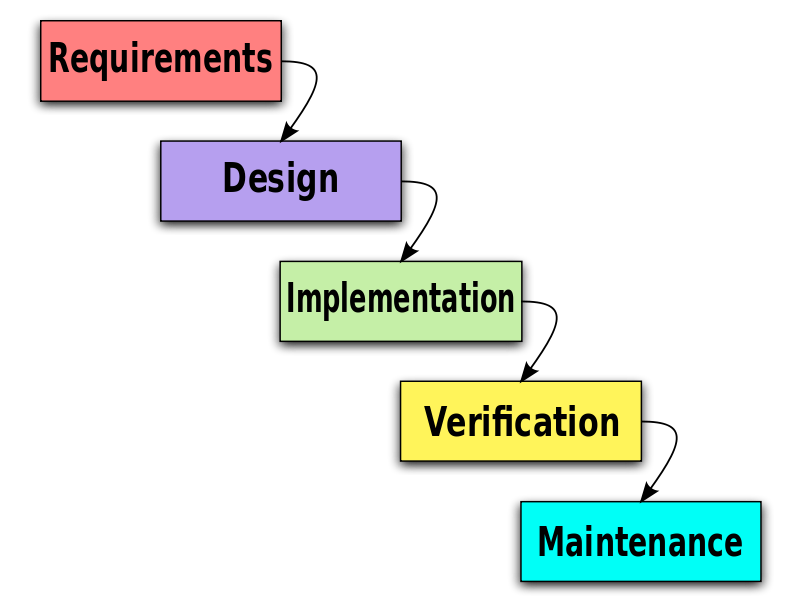
\includegraphics[width=90mm]{graphics/Waterfall_model.png}
\caption{Waterfall Method}
\label{overflow}
\end{figure}

\subsection*{Waterfall Phases:}

\textemdash \textbf{Requirements:} The first step in this methodology to start with requirement analysis and revise in the project is actually feasible with this methodology.

\textbullet \textbf{Design:} With the requirements and analysis acquire in the preview step, them a proper implementation strategy can be formulated according to the software environment. Further the design phase is divided in two sections. \textit{system design and component design}. The system design contains details and specifications of the whole system and explains how each component of the system will interact with others. The component design contains specifications as to how each component will work separately.

\textbullet \textbf{Implementation:} In this phase is where actually some components start being created. The information collected in previews phases are applied in this step to create a functional software.

\textbullet \textbf{Testing:} This step is where the software developed in the preview phase is tested for any errors or discrepancies. In the Waterfall method the testing normally starts when the code is finished.

\textbullet \textbf{Installation:} After the software is tested, it can follow to the next phase where it gets installed in the computer or devices that it is build for.

\textbullet \textbf{Maintenance:} This final phase it could be stretched it for a few month or some years. With this follow up software bugs are fixed and adding/changing additional requirements or functionality to the software.


\section*{Advantages and Disadvantages}

\subsection*{Advantages:} Since the waterfall method is the oldest and most widely used among software development companies there some advantages to this model:
\begin{enumerate}
	\item\ Since it is a linear model, is very simple to implement.
	\item\ The amount of resources to implement it are minimal.
	\item\ Each stage is assigned to separate teams, this approach ensure project deadlines control.
	\item\ Since the documentation is produced at every stage of the software development, this makes its understandably simpler.
	\item\ After every major phase of software programming, testing is done tp the correct runtime.
	\item\ Defined start and end points for each phase of the process, making it more easy to measured. 
\end{enumerate}

\subsection*{Disadvantages:} 
\begin{enumerate}
	\item\ Fixed requirements difficult to change.
	\item\ No final user visibility of the software until the development phase has been completed.
	\item\ Clients are not very clear of what they want exactly from the software, when changes are mention in between it may cause a lot confusion.
	\item\ Small changes or errors that may come up in the final software could cause a lot problems.
\end{enumerate}

The waterfall works really well for commercial arrangements, but when working for internal customers its more difficult to implement.

\section*{Usage}
\textbf{TO BE DONE HERE}


